plot box ratio                            /.initial                 
plot coordinates/math parser              /.is if
plot file       /ignore first             /.style
plot file                                 /.search also             
plot file       /skip first               /.default
plot file       /skip first               /.is if
plot graphics   /auto adjust axis         /.is if
plot graphics                             /.code                    
plot graphics   /debug                    /.default
plot graphics   /debug                    /.initial
plot graphics   /includegraphics cmd      /.initial
plot graphics   /includegraphics          /.initial
plot graphics   /lowlevel draw            /.code 2 args
plot graphics   /lowlevel get natural size/.code
plot graphics   /node                     /.style
plot graphics   /points                   /.initial
plot graphics   /snap z                   /.initial
plot graphics   /squeeze tol              /.initial
plot graphics   /src                      /.initial
plot graphics   /xmax                     /.initial
plot graphics   /xmin                     /.initial
plot graphics   /ymax                     /.initial
plot graphics   /ymin                     /.initial
plot graphics   /zmax                     /.initial
plot graphics   /zmin                     /.initial
plot shift auto                           /.style args              
plot xshift auto                          /.style 2 args            
plot yshift auto                          /.style 2 args            

 \begin{document} 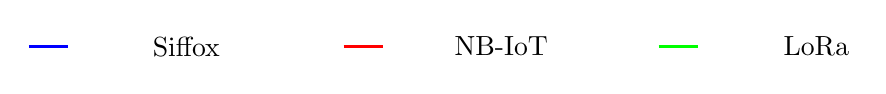
\begin{tikzpicture} \tkzKiviatDiagramFromFile[ scale = .5, label distance = .5cm, gap = 1, label space = 3, lattice = 6]{tableae.dat} \tkzKiviatLineFromFile[thick, color = green, mark = ball, ball color = green, mark size = 4pt, fill = green!20]{tableae.dat}{3} \tkzKiviatLineFromFile[thick, color = blue, mark = ball, ball color = blue, mark size = 4pt, fill = blue!20]{tableae.dat}{2} \tkzKiviatLineFromFile[thick, color = red, mark = ball, ball color = red, mark size = 4pt, fill = red!20]{tableae.dat}{1} \draw [thick, blue] (-6,-11) -- (-5.5,-11); \node at (-4,-11) {Siffox}; \draw [thick, red] (-2,-11) -- (-1.5,-11); \node at (0,-11) {NB-IoT}; \draw [thick, green] (2,-11) -- (2.5,-11); \node at (4,-11) {LoRa}; \end{tikzpicture} \end{document}
